\chapter{Directed graphs}\label{chap:digraphs}

\section{Definitions}

So far, we have been working with graphs with undirected edges.  A
\emph{directed edge} is an edge where the endpoints are
distinguished---one is the \emph{head} and one is the \emph{tail}.  In
particular, a directed edge is specified as an ordered pair of
vertices $u$, $v$ and is denoted by~$(u, v)$ or $\diredge{u}{v}$.  In this
case, $u$ is the \term{tail} of the edge and $v$ is the \term{head}.
For example, see Figure~\ref{fig:6EA}.

\begin{figure}

\begin{equation*}
    {}_u^{\text{tail}} \bullet \to \bullet_v^{\text{head}}
\end{equation*}

\missinggraphic

\caption{A directed edge $e = (u, v)$.  \ $u$ is the tail of~$e$ and
  $v$ is the head of~$e$.}

\label{fig:6EA}
\end{figure}

A graph with directed edges is called a \emph{directed graph} or
\emph{digraph}.

\begin{definition}\label{def:digraph}
A directed graph $G = (V, E)$ consists of a nonempty set of nodes~$V$
and a set of directed edges~$E$.  Each edge~$e$ of~$E$ is specified by
an ordered pair of vertices $u, v \in V$.  A directed graph
is \emph{simple} if it has no \emph{loops} (that is, edges of the form
$\diredge{u}{u}$) and no multiple edges.
\end{definition}

Since we will focus on the case of simple directed graphs in this
chapter, we will generally omit the word \emph{simple} when referring
to them.  Note that such a graph can contain an edge $\diredge{u}{v}$
as well as the edge $\diredge{v}{u}$ since these are different edges
(for example, they have a different tail).

Directed graphs arise in applications where the relationship
represented by an edge is 1-way or asymmetric.  Examples include: a
1-way street, one person likes another but the feeling is not
necessarily reciprocated, a communication channel such as a cable
modem that has more capacity for downloading than uploading, one
entity is larger than another, and one job needs to be completed
before another job can begin. We'll see several such examples in this
chapter and also in Chapter~\ref{chap:partial_orders}.

Most all of the definitions for undirected graphs from
Chapter~\ref{chap:graph_theory} carry over in a natural way for
directed graphs.  For example, two directed graphs $G_1 = (V_1, E_1)$
and $G_2 = (V_2, E_2)$ are \emph{isomorphic} if there exists a
bijection $f: V_1 \to V_2$ such that for every pair of vertices $u, v
\in V_1$,
\begin{equation*}
    \diredge{u}{v} \in E_1 \qquad \QIFF \qquad \diredge{f(u)}{f(v)} \in E_2.
\end{equation*}

Directed graphs have adjacency matrices just like undirected graphs.
In the case of a directed graph $G = (V, E)$, the adjacency matrix
$A_G = \set{ a_{ij} }$ is defined so that
\begin{equation*}
    a_{ij} = \begin{cases}
                1 & \text{if $\diredge{i}{j} \in E$} \\
                0 & \text{otherwise.}
              \end{cases}
\end{equation*}
The only difference is that the adjacency matrix for a directed graph
is not necessarily symmetric (that is, it may be that
$A_{G}^{T} \ne A_G$).

\subsection{Degrees}

With directed graphs, the notion of degree splits into \emph{indegree}
and \emph{outdegree}.  For example, $\indegr{c} = 2$ and $\outdegr{c}
= 1$ for the graph in Figure~\ref{fig:6EB}.  If a node has
outdegree~0, it is called a \emph{sink}; if it has indegree~0, it is
called a \emph{source}.  The graph in Figure~\ref{fig:6EB} has one
source (node~$a$) and no sinks.

\begin{figure}

\missinggraphic

\caption{A 4-node directed graph with 6 edges.}

\label{fig:6EB}

\end{figure}

\subsection{Directed Walks, Paths, and Cycles}

The definitions for (directed) walks, paths, and cycles in a directed
graph are similar to those for undirected graphs except that the
direction of the edges need to be consistent with the order in which
the walk is traversed.

\begin{definition}

A \emph{directed walk} (or more simply, a \emph{walk}) in a directed
graph~$G$ is a sequence of vertices $v_0$, $v_1$, \dots, $v_k$ and
edges
\begin{equation*}
    \diredge{v_0}{v_1}, \diredge{v_1}{v_2}, \dots, \diredge{v_{k - 1}}{v_k}
\end{equation*}
such that $\diredge{v_{i - 1}}{v_i}$ is an edge of~$G$ for all~$i$ where $0
\le i < k$.  A \emph{directed path} (or \emph{path}) in a directed
graph is a walk where the nodes in the walk are all different.  A
\emph{directed closed walk} (or \emph{closed walk}) in a directed
graph is a walk where $v_0 = v_k$.  A \emph{directed cycle} (or
\emph{cycle}) in a directed graph is a closed walk where all the
vertices~$v_i$ are different for $0 \le i < k$.
\end{definition}

As with undirected graphs, we will typically refer to a walk in a
directed graph by a sequence of vertices.  For example, for the graph
in Figure~\ref{fig:6EB},
\begin{itemize}

\item
$a$, $b$, $c$, $b$, $d$ is a walk,

\item
$a$, $b$, $d$ is a path,

\item
$d$, $c$, $b$, $c$, $b$, $d$ is a closed walk, and

\item
$b$, $d$, $c$, $b$ is a cycle.

\end{itemize}

Note that $b$, $c$, $b$ is also a cycle for the graph in
Figure~\ref{fig:6EB}.  This is a cycle of length~2.  Such cycles are
not possible with undirected graphs.

Also note that
\begin{equation*}
    c, b, a, d
\end{equation*}
is \emph{not} a walk in the graph shown in Figure~\ref{fig:6EB}, since
$\diredge{b}{a}$ is not an edge in this graph.  (You are \emph{not}
allowed to traverse edges in the wrong direction as part of a walk.)

A path or cycle in a directed graph is said to be \emph{Hamiltonian}
if it visits every node in the graph.  For example, $a$, $b$, $d$, $c$
is the only Hamiltonian path for the graph in Figure~\ref{fig:6EB}.
The graph in Figure~\ref{fig:6EB} does not have a Hamiltonian cycle.

A walk in a directed graph is said to be \emph{Eulerian} if it
contains every edge.  The graph shown in Figure~\ref{fig:6EB} does not
have an Eulerian walk.  Can you see why not?  (Hint: Look at
node~$a$.)

\subsection{Strong Connectivity}

The notion of being connected is a little more complicated for a
directed graph than it is for an undirected graph.  For example,
should we consider the graph in Figure~\ref{fig:6EB} to be connected?
There is a path from node~$a$ to every other node so on that basis, we
might answer ``Yes.''  But there is no path from nodes $b$, $c$,
or~$d$ to node~$a$, and so on that basis, we might answer ``No.''  For
this reason, graph theorists have come up with the notion of
\emph{strong} connectivity for directed graphs.

\begin{definition}
A directed graph $G = (V, E)$ is said to be \emph{strongly connected}
if for every pair of nodes $u, v \in V$, there is a directed path from
$u$ to~$v$ (and vice-versa) in~$G$.
\end{definition}

For example, the graph in Figure~\ref{fig:6EB} is not strongly
connected since there is no directed path from node~$b$ to node~$a$.
But if node~$a$ is removed, the resulting graph would be strongly
connected.

A directed graph is said to be \emph{weakly connected} (or, more
simply, \emph{connected}) if the corresponding undirected graph (where
directed edges $\diredge{u}{v}$ and/or $\diredge{v}{u}$ are replaced
with a single undirected edge $\edge{u}{v}$) is connected.  For example,
the graph in Figure~\ref{fig:6EB} is weakly connected.

\subsection{DAGs}

If an undirected graph does not have any cycles, then it is a tree or
a forest.  But what does a directed graph look like if it has no
cycles?  For example, consider the graph in Figure~\ref{fig:6ED}.
This graph is weakly connected and has no directed cycles but it
certainly does not look like a tree.

\begin{figure}

\missinggraphic

\caption{A 4-node directed acyclic graph (DAG).}

\label{fig:6ED}

\end{figure}

\begin{definition}
A directed graph is called a \emph{directed acyclic graph} (or,
\emph{DAG}) if it does not contain any directed cycles.
\end{definition}

A first glance, DAGs don't appear to be particularly interesting.  But
first impressions are not always accurate.  In fact, DAGs arise in
many scheduling and optimization problems and they have several
interesting properties.  We will study them extensively in
Chapter~\ref{chap:partial_orders}.

\section{Tournament Graphs}

Suppose that $n$ players compete in a round-robin tournament and that
for every pair of players $u$ and~$v$, either $u$ beats~$v$ or $v$
beats~$u$.  Interpreting the results of a round-robin tournament can
be problematic---there might be all sorts of cycles where $x$
beats~$y$ and $y$ beats $z$, yet $z$ beats~$x$.  Who is the best
player?  Graph theory does not solve this problem but it can provide
some interesting perspectives.

The results of a round-robin tournament can be represented with a
\term{tournament graph}.  This is a directed graph in which the
vertices represent players and the edges indicate the outcomes of
games.  In particular, an edge from $u$ to~$v$ indicates that
player~$u$ defeated player~$v$.  In a round-robin tournament, every
pair of players has a match.  Thus, in a tournament graph there is
either an edge from $u$ to~$v$ or an edge from $v$ to~$u$ (but not
both) for \emph{every} pair of distinct vertices $u$ and~$v$.  An
example of a tournament graph is shown in Figure~\ref{fig:6EE1}.

\begin{figure}

\missinggraphic

\caption{A 5-node tournament graph.}

\label{fig:6EE1}

\end{figure}

\subsection{Finding a Hamiltonian Path in a Tournament Graph}

We're going to prove that in every round-robin tournament, there
exists a ranking of the players such that each player lost to the
player one position higher.  For example, in the tournament
corresponding to Figure~\ref{fig:6EE1}, the ranking
\begin{equation*}
    a > b > d > e > c
\end{equation*}
satisfies this criterion, because $b$ lost to~$a$, \ $d$ lost to~$b$,
\ $e$ lost to~$d$, and $c$ lost to~$e$.  In graph terms, proving the
existence of such a ranking amounts to proving that every tournament
graph has a Hamiltonian path.

\begin{theorem}\label{thm:hamilton_tournament}
Every tournament graph contains a directed Hamiltonian path.
\end{theorem}

\begin{proof}

We use strong induction.  Let $P(n)$ be the proposition that every
tournament graph with $n$ vertices contains a directed Hamiltonian
path.

\inductioncase{Base case}: $P(1)$ is trivially true; every graph with
a single vertex has a Hamiltonian path consisting of only that vertex.

\inductioncase{Inductive step}: For $n \ge 1$, we assume that $P(1)$,
\dots, $P(n)$ are all true and prove $P(n + 1)$.  Consider a
tournament graph $G = (V, E)$ with $n + 1$ players.  Select one
vertex~$v$ arbitrarily.  Every other vertex in the tournament either
has an edge \emph{to} vertex~$v$ or an edge \emph{from} vertex~$v$.
Thus, we can partition the remaining vertices into two corresponding
sets, $T$ and~$F$, each containing at most $n$ vertices, where $T =
\set{\, u \mid \diredge{u}{v} \in E \,}$ and
$F = \set{\, u \mid \diredge{v}{u} \in E \,}$.
For example, see Figure~\ref{fig:6EE2}.

\begin{figure}

\missinggraphic

\caption{The sets $T$ and~$F$ in a tournament graph.}

\label{fig:6EE2}

\end{figure}

The vertices in~$T$ together with the edges that join them form a
smaller tournament.  Thus, by strong induction, there is a Hamiltonian
path within~$T$.  Similarly, there is a Hamiltonian path within the
tournament on the vertices in~$F$.  Joining the path in~$T$ to the
vertex~$v$ followed by the path in~$F$ gives a Hamiltonian path
through the whole tournament.  As special cases, if $T$ or~$F$ is
empty, then so is the corresponding portion of the path.
\end{proof}

The ranking defined by a Hamiltonian path is not entirely
satisfactory.  For example, in the tournament associated with
Figure~\ref{fig:6EE1}, notice that the lowest-ranked player,~$c$,
actually defeated the highest-ranked player,~$a$.

In practice, players are typically ranked according to how many
victories they achieve.  This makes sense for several reasons.  One
not-so-obvious reason is that if the player with the most victories
does not beat some other player~$v$, he is guaranteed to have at least
beaten a third player who beat~$v$.  We'll prove this fact shortly,
but first, let's talk about chickens.

\subsection{The King Chicken Theorem}

Suppose that there are $n$ chickens in a farmyard.  Chickens are
rather aggressive birds that tend to establish dominance in
relationships by pecking.  (Hence the term ``pecking order.'')  In
particular, for each pair of distinct chickens, either the first pecks
the second or the second pecks the first, but not both.  We say that
chicken~$u$ \emph{virtually pecks} chicken~$v$ if either:
\begin{itemize}

\item Chicken $u$ directly pecks chicken~$v$, or

\item Chicken $u$ pecks some other chicken~$w$ who in turn pecks
  chicken~$v$.

\end{itemize}
A chicken that virtually pecks every other chicken is called a
\emph{king chicken}.

We can model this situation with a tournament digraph.  The vertices
are chickens, and an edge $\diredge{u}{v}$ indicates that chicken~$u$ pecks
chicken~$v$.  In the tournament shown in Figure~\ref{fig:6EE3}, three
of the four chickens are kings.  Chicken~$c$ is not a king in this
example since it does not peck chicken~$b$ and it does not peck any
chicken that pecks chicken~$b$.  Chicken~$a$ \emph{is} a king since it
pecks chicken~$d$, who in turn pecks chickens $b$ and~$c$.

\begin{figure}

\missinggraphic

\caption{A 4-chicken tournament in which chickens $a$, $b$, and~$d$
  are kings.}

\label{fig:6EE3}.

\end{figure}

\begin{theorem}[King Chicken Theorem]\label{thm:king_chicken}
The \dmj{A?} chicken with the highest \dmj{maximum?} outdegree
in an $n$-chicken tournament is a king.
\end{theorem}

\begin{proof}
By contradiction.  Let $u$ be a node in a tournament graph $G = (V,
E)$ with maximum outdegree and suppose that $u$ is not a king.  Let $Y
= \set{\, v \mid \diredge{u}{v} \in E \,}$ be the set of chickens that
chicken~$u$ pecks.  Then $\outdegr{u} = \card{Y}$.

Since $u$ is not a king, there is a chicken $x \notin Y$ (that is, $x$
is not pecked by chicken~$u$) and that is not pecked by any chicken
in~$Y$.  Since for any pair of chickens, one pecks the other, this
means that $x$ pecks~$u$ as well as every chicken in~$Y$.  This means
that
\begin{align*}
    \outdegr{x} &= \card{Y} + 1 \\
                &> \outdegr{u}.
\end{align*}

But $u$ was assumed to be the node with the highest degree in the
tournament, so we have a contradiction.  Hence, $u$ must be a king.
\end{proof}

Theorem~\ref{thm:king_chicken} means that if the player with the most
victories is defeated by another player~$x$, then at least he/she
defeats some third player that defeats~$x$.  In this sense, the player
with the most victories has some sort of bragging rights over every
other player.  Unfortunately, as Figure~\ref{fig:6EE3} illustrates,
there can be many other players with such bragging rights, even some
with fewer victories.  Indeed, for some tournaments, it is possible
that every player is a ``king.''  For example, consider the tournament
illustrated in Figure~\ref{fig:6EE4}.

\begin{figure}

\missinggraphic

\caption{A 5-chicken tournament in which every chicken is a king.}

\label{fig:6EE4}

\end{figure}

\section{Communication
  Networks}\label{comm_net_sec}\label{chap:comm_nets}

While reasoning about chickens pecking each other may be amusing (to
mathematicians, at least), the use of directed graphs to model
communication networks is very serious business.  In the context of
communication problems, vertices represent computers, processors, or
switches, and edges represent wires, fiber, or other transmission
lines through which data flows.  For some communication networks, like
the Internet, the corresponding graph is enormous and largely chaotic.
Highly structured networks, such as an array or butterfly, by
contrast, find application in telephone switching systems and the
communication hardware inside parallel computers.

\subsection{Packet Routing}

Whatever architecture is chosen, the goal of a communication network
is to get data from \emph{inputs} to \emph{outputs}.  In this text, we
will focus on a model in which the data to be communicated is in the
form of a \emph{packet}.  In practice, a packet would consist of a
fixed amount of data, and a message (such as a web page or a movie)
would consist of many packets.

For simplicity, we will restrict our attention to the scenario where
there is just one packet at every input and where there is just one
packet destined for each output.  We will denote the number of inputs
and output by~$N$ and we will often assume that $N$ is a power of two.

We will specify the desired destinations of the packets by a
permutation\footnote{A permutation of a sequence is a reordering of
  the sequence.} of 0, 1, \dots, $N - 1$.  So a permutation, $\pi$,
defines a \emph{routing problem}: get a packet that starts at
input~$i$ to output~$\pi(i)$ for $0 \le i < N$.  A \emph{routing},
$P$, that \emph{solves} a routing problem, $\pi$, is a set of paths
from each input to its specified output.  That is, $P$ is a set of
paths, $P_i$, for $i = 0, \dots, N - 1$, where $P_i$ goes from
input~$i$ to output~$\pi(i)$.

Of course, the goal is to get all the packets to their destinations as
quickly as possible using as little hardware as possible.  The time
needed to get the packages to their destinations depends on several
factors, such as how many switches they need to go through and how
many packets will need to cross the same wire.  We will assume that
only one packet can cross a wire at a time.  The complexity of the
hardware depends on factors such as the number of switches needed and
the size of the switches.

Let's see how all this works with an example---routing packets on a
complete binary tree.

\subsection{The Complete Binary Tree}

One of the simplest structured communications networks is a
\emph{complete binary tree}.  A complete binary tree with 4 inputs and
4 outputs is shown in Figure~\ref{fig:6EH}.

\begin{figure}

\missinggraphic

\caption{A 4-input, 4-output complete binary tree.  The squares
  represent terminals (input and output registers) and the circles
  represent switches.  Directed edges represent communication channels
  in the network through which data packets can move.  The unique path
  from input~1 to output~3 is shown in bold.}

\label{fig:6EH}

\end{figure}

In this diagram and many that follow, the squares represent
\term{terminals} (that is, the inputs and outputs), and the circles
represent \term{switches}, which direct packets through the network.
A switch receives packets on incoming edges and relays them forward
along the outgoing edges.  Thus, you can imagine a data packet hopping
through the network from an input terminal, through a sequence of
switches joined by directed edges, to an output terminal.

Recall that there is a unique simple path between every pair of
vertices in a tree.  So the natural way to route a packet of data from
an input terminal to an output terminal in the complete binary tree is
along the corresponding directed path.  For example, the route of a
packet traveling from input~1 to output~3 is shown in bold in
Figure~\ref{fig:6EH}.

\subsection{Network Diameter}

The delay between the time that a packet arrives at an input and the
time it reaches its designated output is referred to as \term{latency}
and it is a critical issue in communication networks.  If congestion
is not a factor, then this delay is generally proportional to the
length of the path a packet follows.  Assuming it takes one time unit
to travel across a wire, and that there are no additional delays at
switches, the delay of a packet will be the number of wires it crosses
going from input to output.\footnote{Latency can also be measured as
  the number of switches that a packet must pass through when
  traveling between the most distant input and output, since switches
  usually have the biggest impact on network speed.  For example, in
  the complete binary tree example, the packet traveling from input 1
  to output 3 crosses 5 switches, which is 1 less than the number of
  edges traversed.}

Generally a packet is routed from input to output using the shortest
path possible.  The length of this shortest path is the
\term{distance} between the input and output.  With a shortest path
routing, the worst possible delay is the distance between the input
and output that are farthest apart.  This is called the
\term{diameter} of the network.  In other words, the diameter of a
network\footnote{The usual definition of \emph{diameter} for a general
  graph (simple or directed) is the largest distance between
  \emph{any} two vertices, but in the context of a communication
  network, we're only interested in the distance between inputs and
  outputs, not between arbitrary pairs of vertices.} is the maximum
length of any shortest path between an input and an output.  For
example, in the complete binary tree shown in Figure~\ref{fig:6EH},
the distance from input~1 to output~3 is six.  No input and output are
farther apart than this, so the diameter of this tree is also six.

More generally, the diameter of a complete binary tree with $N$ inputs
and outputs is $2 \log N + 2$.  (All logarithms in this lecture---and
in most of computer science---are base 2.)  This is quite good,
because the logarithm function grows very slowly.  We could connect
$2^{20} = 1{,}048{,}576$ inputs and outputs using a complete binary
tree and the worst input-output delay for any packet would be this
diameter, namely, $2 \log(2^{20}) + 2 = 42$.

\subsection{Switch Size}

One way to reduce the diameter of a network (and hence the latency
needed to route packets) is to use larger switches.  For example, in
the complete binary tree, most of the switches have three incoming
edges and three outgoing edges, which makes them $3 \times 3$
switches.  If we had $4 \times 4$ switches, then we could construct a
complete \emph{ternary} tree with an even smaller diameter.  In
principle, we could even connect up all the inputs and outputs via a
single monster $N \times N$ switch, as shown in Figure~\ref{fig:6EI}.
In this case, the ``network'' would consist of a single switch and the
latency would be~2.

\begin{figure}

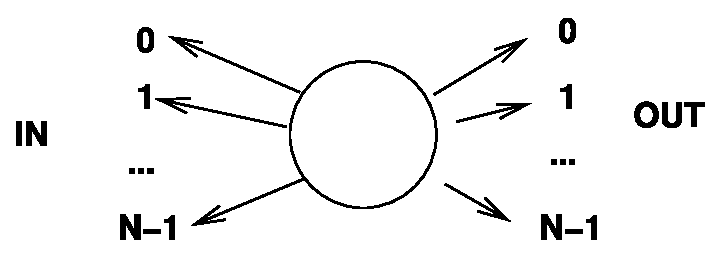
\includegraphics[height=1in]{monster-switch}

\missinggraphic[Fix labels]

\caption{A monster $N \by N$ switch.}

\label{fig:6EI}

\end{figure}

This isn't very productive, however, since we've just concealed the
original network design problem inside this abstract monster switch.
Eventually, we'll have to design the internals of the monster switch
using simpler components, and then we're right back where we started.
So the challenge in designing a communication network is figuring out
how to get the functionality of an $N \times N$ switch using fixed
size, elementary devices, like $3 \times 3$ switches.
\begin{solution}
Following this approach, we can build arbitrarily large networks
just by adding in more building blocks. 
\end{solution}

\subsection{Switch Count}

Another goal in designing a communication network is to use as few
switches as possible.  The number of switches in a complete binary
tree is $1 + 2 + 4 + 8 + \cdots + N = 2N - 1$, since there is 1 switch
at the top (the ``root switch''), 2 below it, 4 below those, and so
forth.  This is nearly the best possible with $3 \times 3$ switches,
since at least one switch will be needed for each pair of inputs and
outputs.

\subsection{Congestion}

The complete binary tree has a fatal drawback: the root switch is a
bottleneck.  At best, this switch must handle an enormous amount of
traffic: every packet traveling from the left side of the network to the
right or vice-versa.  Passing all these packets through a single switch
could take a long time.  At worst, if this switch fails, the network is
broken into two equal-sized pieces.

The traffic through the root depends on the routing problem.  For
example, if the routing problem is given by the identity permutation,
\dmj{Is ``Id'' suppose to change?} $\ident{}(i) \eqdef i$, then
there is an easy routing, $P$, that solves the problem: let $P_i$ be
the path from input $i$ up through one switch and back down to output
$i$.  On the other hand, if the problem was given by $\pi(i) \eqdef (N
- 1) - i$, then in \emph{any} solution, $P$, for $\pi$, each path
$P_i$ beginning at input $i$ must eventually loop all the way up
through the root switch and then travel back down to output $(N - 1) -
i$.  These two situations are illustrated in Figure~\ref{fig:6EJ}.

\begin{figure}
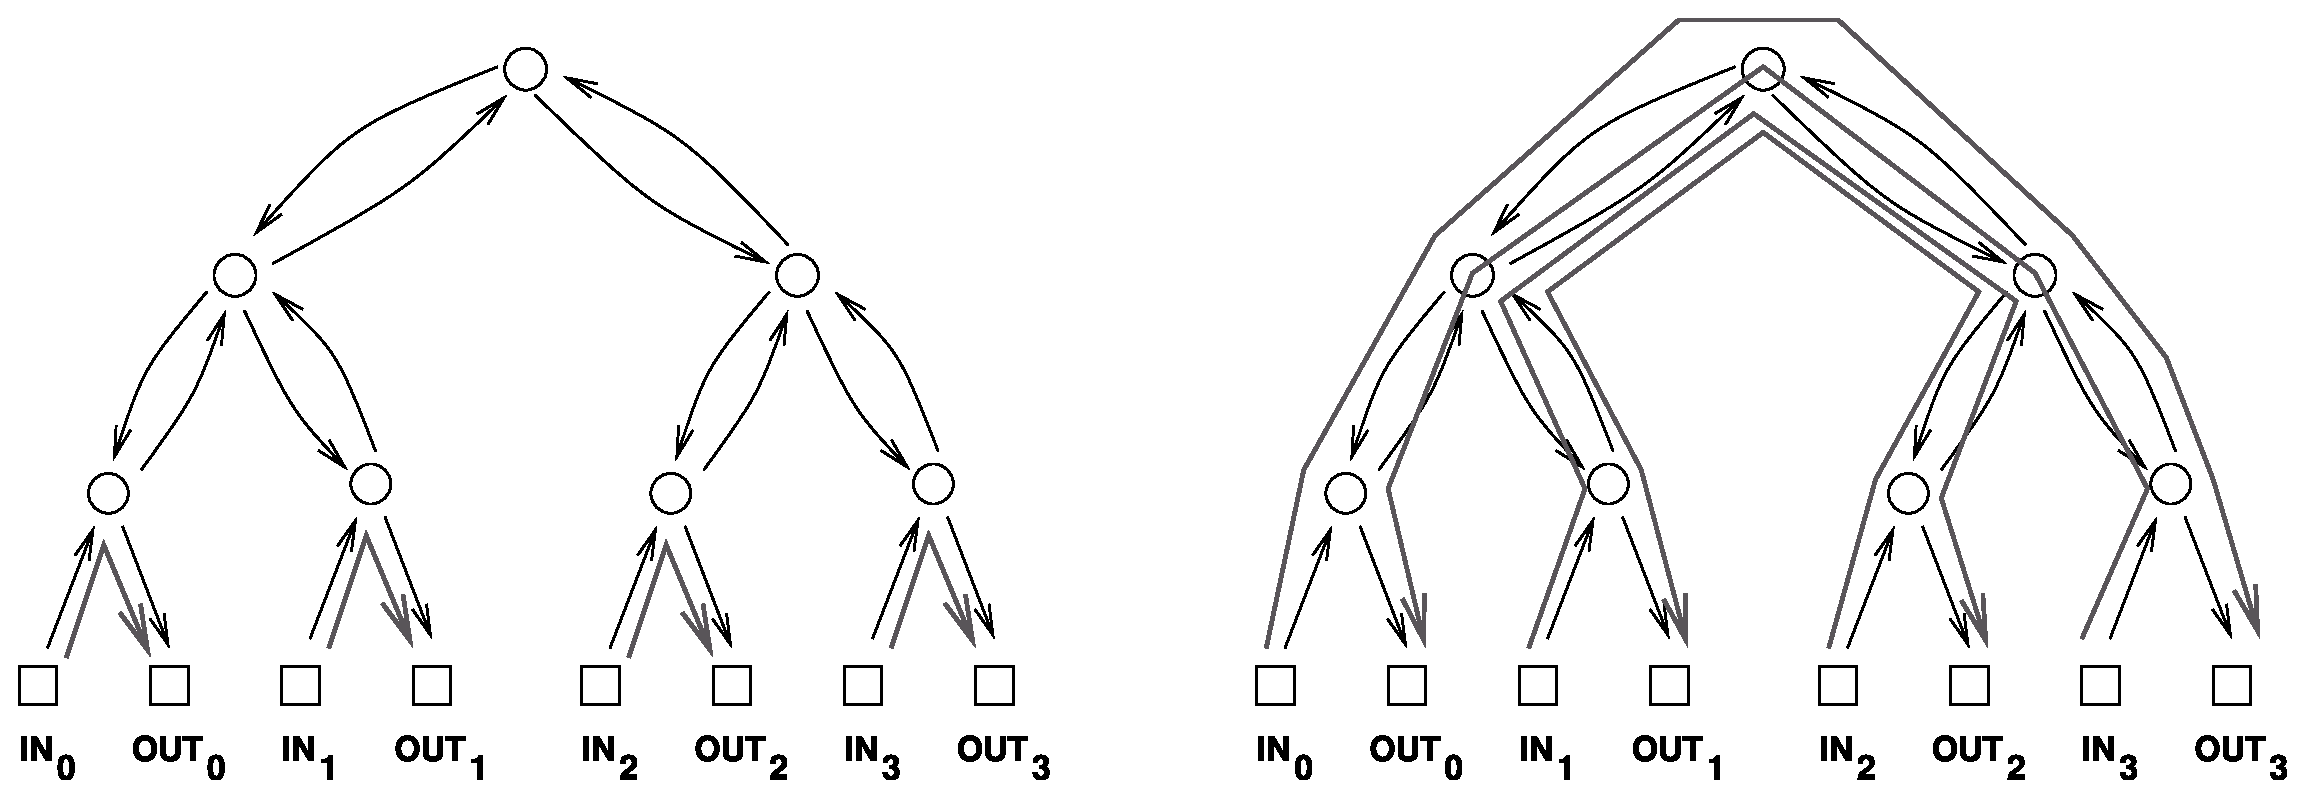
\includegraphics[height=1.5in]{bintree2}

\missinggraphic[Split into to two subfigures]

\caption{Paths for the routing problem given by $\pi(i) = i$~(a) and
  $\pi(i) = N - 1 - i$~(b).  The root is a bottleneck in the latter
  scenario.}

\label{fig:6EJ}

\end{figure}

We can distinguish between a ``good'' set of paths and a ``bad'' set
based on congestion.  The \term{congestion} of a routing, $P$, is
equal to the largest number of paths in $P$ that pass through a single
switch.  For example, the congestion of the routing in
Figure~\ref{fig:6EJ}(a) is~1, since at most 1 path passes through each
switch.  However, the congestion of the routing in
Figure~\ref{fig:6EJ}(b) is~4, since 4 paths pass through the root
switch (and the two switches directly below the root).  Generally,
lower congestion is better since packets can be delayed at an
overloaded switch.

By extending the notion of congestion to networks, we can also distinguish
between ``good'' and ``bad'' networks with respect to bottleneck problems.
For each routing problem, $\pi$, for the network, we assume a routing is
chosen that optimizes congestion, that is, that has the minimum congestion
among all routings that solve $\pi$.  Then the largest congestion that
will ever be suffered by a switch will be the maximum congestion among
these optimal routings.  This ``maxi-min'' congestion is called the
\term{congestion of the network}.

You may find it helpful to think about max congestion in terms of a
value game.  You design your spiffy, new communication network; this
defines the game.  Your opponent makes the first move in the game: she
inspects your network and specifies a permutation routing problem that
will strain your network.  You move second: given her specification,
you choose the precise paths that the packets should take through your
network; you're trying to avoid overloading any one switch.  Then her
next move is to pick a switch with as large as possible a number of
packets passing through it; this number is her score in the
competition.  The max congestion of your network is the largest score
she can ensure; in other words, it is precisely the max-value of this
game.

For example, if your enemy were trying to defeat the complete binary
tree, she would choose a permutation like $\pi(i) = (N - 1) - i$.
Then for \emph{every} packet $i$, you would be forced to select a path
$P_{i, \pi(i)}$ passing through the root switch.  Then, your enemy
would choose the root switch and achieve a score of~$N$.  In other
words, the max congestion of the complete binary tree is $N$---which
is horrible!

We have summarized the results of our analysis of the complete binary
tree in Figure~\ref{fig:6EK}.  Overall, the complete binary tree does
well in every category except the last---congestion, and that is a
killer in practice.  Next, we will look at a network that solves the
congestion problem, but at a very high cost.

\begin{figure}

\begin{tabular}{r|c|c|c|c}
\textbf{network} &
\textbf{diameter} &
\textbf{switch size} &
\textbf{\# switches} &
\textbf{congestion} \\ \hline
complete binary tree & $2 \log N + 2$ & $3 \times 3$ & $2N - 1$ & $N$
\end{tabular}

\caption{A summary of the attributes of the complete binary tree.}

\label{fig:6EK}

\end{figure}

\subsection{The 2-d Array}\label{sec:2d-array}

An illustration of the $N \by N$ 2-d \emph{array} (also known as the
\emph{grid} or \emph{crossbar}) is shown in Figure~\ref{fig:6EL} for
the case when $N = 4$.

\begin{figure}

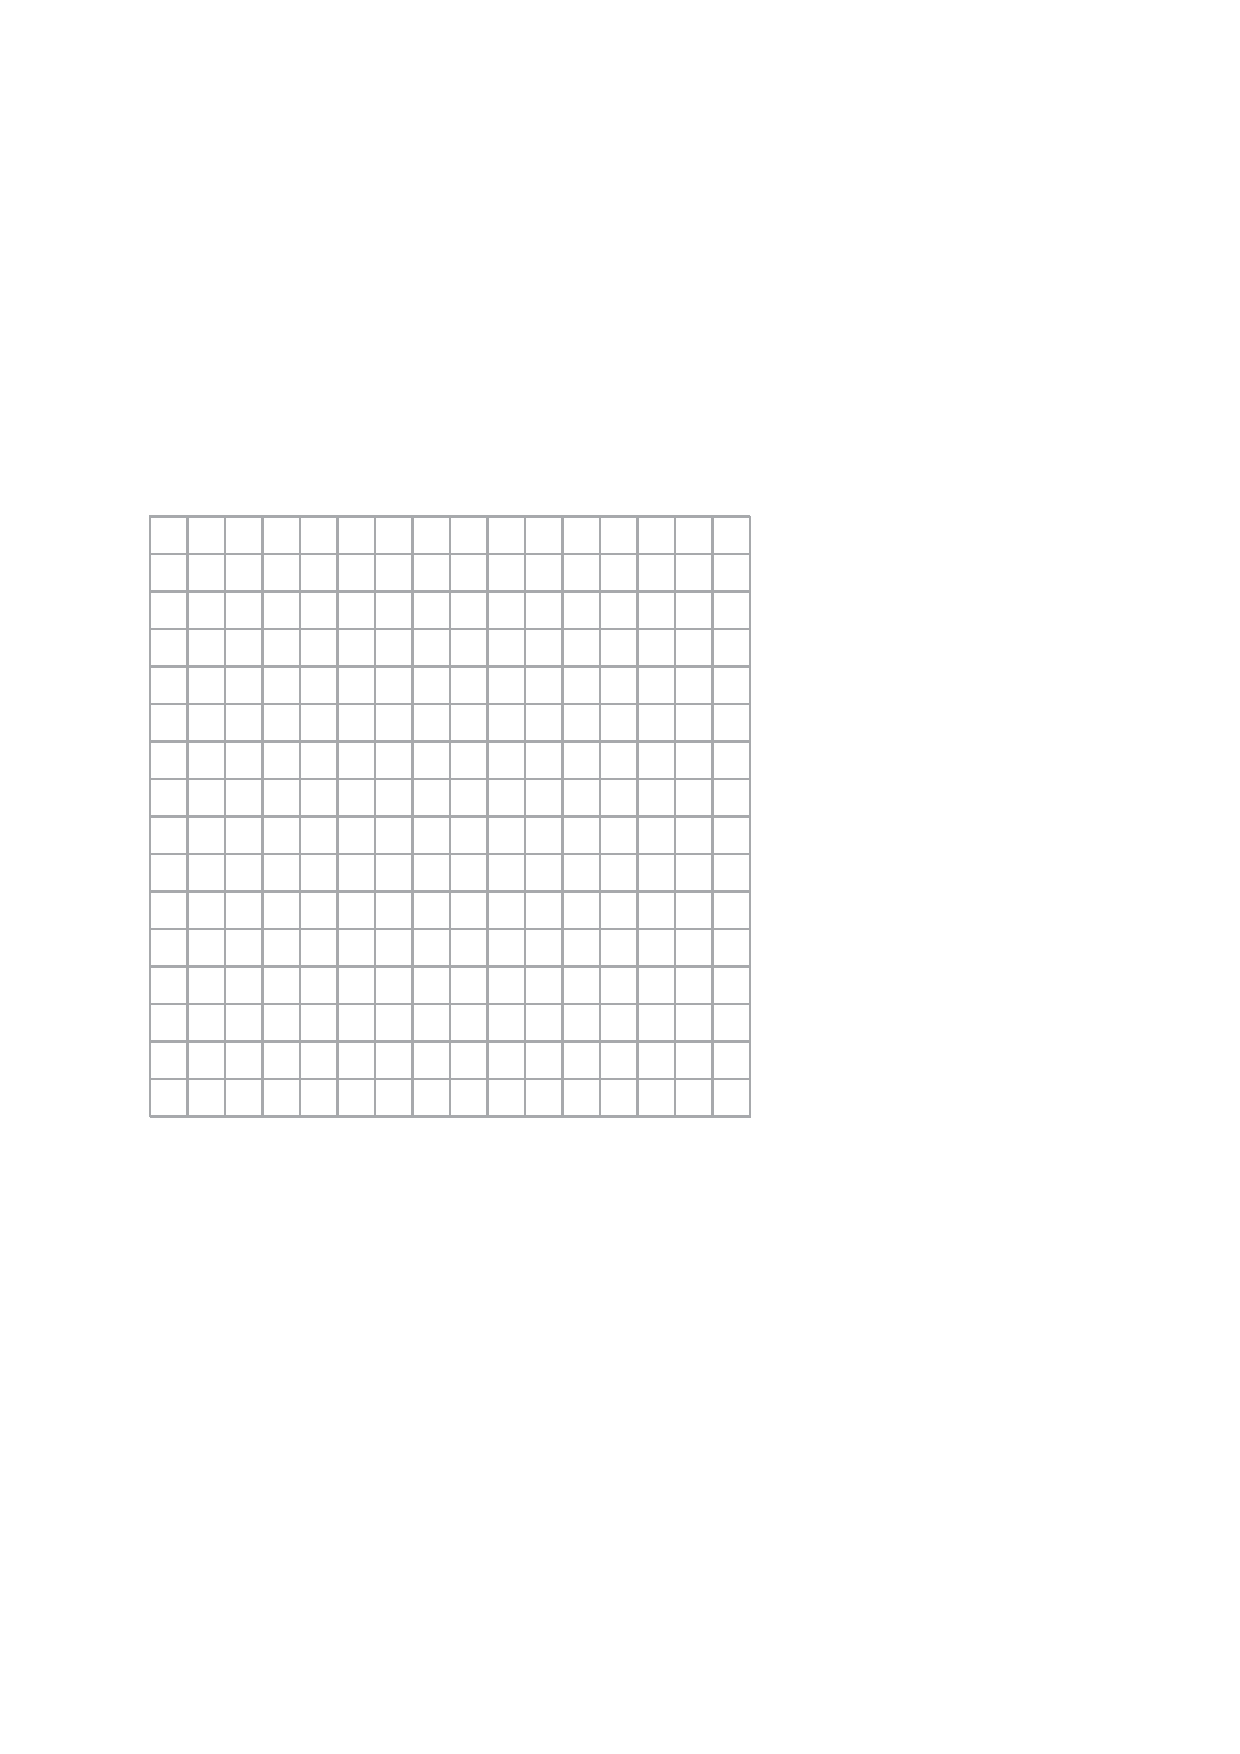
\includegraphics[height=2in]{grid}

\caption{A $4 \by 4$ 2-dimensional array.}

\label{fig:6EL}

\end{figure}

The diameter of the $4 \by 4$ 2-d array is~8, which is the number of
edges between input 0 and output 3.  More generally, the diameter of a
2-d array with $N$ inputs and outputs is $2N$, which is much worse
than the diameter of the complete binary tree ($2 \log N + 2$).  On
the other hand, replacing a complete binary tree with a 2-d array
almost eliminates congestion.

\begin{theorem}
The congestion of an $N$-input 2-d array is~2.
\end{theorem}

\begin{proof}
First, we show that the congestion is at most 2.  Let $\pi$ be any
permutation.  Define a solution, $P$, for $\pi$ to be the set of
paths, $P_i$, where $P_i$ goes to the right from input $i$ to column
$\pi(i)$ and then goes down to output $\pi(i)$.  In this solution, the
switch in row $i$ and column $j$ encounters at most two packets: the
packet originating at input $i$ and the packet destined for output
$j$.

Next, we show that the congestion is at least 2.  This follows because in
any routing problem, $\pi$, where $\pi(0) = 0$ and $\pi(N-1) =
N-1$, two packets must pass through the lower left switch.
\end{proof}

The characteristics of the 2-d array are recorded in
Figure~\ref{fig:6EM}. The crucial entry in this table is the number of
switches, which is $N^2$.  This is a major defect of the 2-d array;
a network with $N = 1000$ inputs would require a \emph{million} $2
\times 2$ switches!  Still, for applications where $N$ is small, the
simplicity and low congestion of the array make it an attractive
choice.


\begin{figure}

\begin{tabular}{r|c|c|c|c}
\textbf{network} &
\textbf{diameter} &
\textbf{switch size} &
\textbf{\# switches} &
\textbf{congestion} \\ \hline
complete binary tree & $2 \log N + 2$ & $3 \times 3$ & $2N - 1$ & $N$ \\
2-D array            & $2 N$          & $2 \times 2$ & $N^2$    & 2
\end{tabular}

\caption{Comparing the $N$-input 2-d array to the $N$-input
  complete binary tree.}

\label{fig:6EM}

\end{figure}

\subsection{The Butterfly}

The Holy Grail of switching networks would combine the best properties
of the complete binary tree (low diameter, few switches) and the array
(low congestion).  The \term{butterfly} is a widely-used compromise
between the two. A butterfly network with $N = 8$ inputs is shown in
Figure~\ref{fig:6EN}.

\begin{figure}

\missinggraphic

\caption{An 8-input/output butterfly.}

\label{fig:6EN}

\end{figure}

The structure of the butterfly is certainly more complicated than that
of the complete binary or 2-d array.  Let's see how it is constructed.

All the terminals and switches in the network are in $N$ rows.  In
particular, input~$i$ is at the left end of row~$i$, and output~$i$ is
at the right end of row~$i$.  Now let's label the rows in
\emph{binary} so that the label on row~$i$ is the binary number
$b_1b_2\dots b_{\log N}$ that represents the integer~$i$.

Between the inputs and outputs, there are $\log(N) + 1$ levels of
switches, numbered from 0 to~$\log N$.  Each level consists of a
column of $N$ switches, one per row.  Thus, each switch in the network
is uniquely identified by a sequence $(b_1$, $b_2$, \dots, $b_{\log
  N}$, $l)$, where $b_1 b_2 \dots b_{\log N}$ is the switch's row in
binary and $l$ is the switch's level.

All that remains is to describe how the switches are connected up.
The basic connection pattern is expressed below in a compact notation:
\begin{equation*}
\begin{array}{lcr}
    &\raisebox{-5pt}{$\nearrow$}& (b_1, b_2, \dots b_{l + 1}, \dots b_{\log N}, l + 1) \\
(b_1, b_2, \dots b_{l + 1}, \dots b_{\log N}, l) &\\
    &\raisebox{5pt}{$\searrow$}& (b_1, b_2, \dots \bar{b_{l + 1}}, \dots b_{\log N}, l + 1) \\
\end{array}
\end{equation*}
This says that there are directed edges from switch $(b_1, b_2, \dots,
b_{\log N}, l)$ to two switches in the next level.  One edges leads to
the switch in the \emph{same} row, and the other edge leads to the
switch in the row obtained by \emph{inverting} the $(l + 1)$st
bit~$b_{l + 1}$.  For example, referring back to the illustration of
the size $N = 8$ butterfly, there is an edge from switch $(0, 0, 0,
0)$ to switch (0, 0, 0, 1), which is in the same row, and to switch
$(1, 0, 0, 1)$, which is in the row obtained by inverting bit $l + 1 =
1$.

The butterfly network has a recursive structure; specifically, a
butterfly of size~$2N$ consists of two butterflies of size~$N$ and one
additional level of switches.  Each switch in the additional level has
directed edges to a corresponding switch in each of the smaller
butterflies.  For example, see Figure~\ref{fig:6EP}.

\begin{figure}

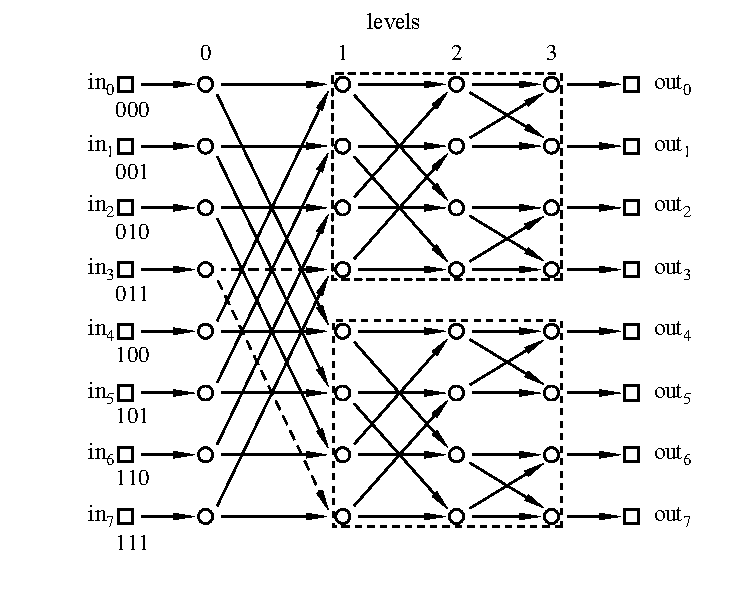
\includegraphics[height=3in]{butterfly3}

\missinggraphic

\caption{An $N$-input butterfly contains two $N/2$-input butterflies
  (shown in the dashed boxes). Each switch on the first level is
  adjacent to a corresponding switch in each of the sub-butterflies.
  For example, we have used dashed lines to show these edges for the
  node $(0, 1, 1, 0)$.}

\label{fig:6EP}

\end{figure}

Despite the relatively complicated structure of the butterfly, there
is a simple way to route packets through its switches.  In particular,
suppose that we want to send a packet from input $x_1 x_2 \dots
x_{\log N}$ to output $y_1 y_2 \dots y_{\log N}$.  (Here we are
specifying the input and output numbers in binary.)  Roughly, the plan
is to ``correct'' the first bit on the first level, correct the second
bit on the second level, and so forth.  Thus, the sequence of switches
visited by the packet is:
%
\begin{align*}
(x_1, x_2, x_3, \dots, x_{\log N}, 0)
    & \to (y_1, x_2, x_3, \dots, x_{\log N}, 1) \\
    & \to (y_1, y_2, x_3, \dots, x_{\log N}, 2) \\
    & \to (y_1, y_2, y_3, \dots, x_{\log N}, 3) \\
    & \to \qquad \dots \\
    & \to (y_1, y_2, y_3, \dots, y_{\log N}, \log N)
\end{align*}
%
In fact, this is the \emph{only} path from the input to the output!

The congestion of the butterfly network is about $\sqrt{N}$.  More
precisely, the congestion is $\sqrt{N}$ if $N$ is an even power of~2
and $\sqrt{N/2}$ if $N$ is an odd power of~2.  The task of proving
this fact has been left to the problem section\footnote{The routing
  problems that result in $\sqrt{N}$ congestion do arise in practice,
  but for most routing problems, the congestion is much lower (around
  $\log N$), which is one reason why the butterfly is useful in
  practice.}.

A comparison of the butterfly with the complete binary tree and the
2-d array is provided in Figure~\ref{fig:6EQ}.  As you can see, the
butterfly has lower congestion than the complete binary tree.  And it
uses fewer switches and has lower diameter than the array.  However,
the butterfly does not capture the best qualities of each network, but
rather is a compromise somewhere between the two.  So our quest for
the Holy Grail of routing networks goes on.

\begin{figure}

\begin{tabular}{r|c|c|c|c}
\textbf{network} &
\textbf{diameter} &
\textbf{switch size} &
\textbf{\# switches} &
\textbf{congestion} \\ \hline
complete binary tree & $2 \log N + 2$ & $3 \times 3$ & $2N - 1$ & $N$ \\
2-D array            & $2 N$          & $2 \times 2$ & $N^2$    & 2 \\
butterfly            & $\log N + 2$ & $2 \times 2$ & $N (\log(N) + 1)$
        & $\sqrt{N}$ or $\sqrt{N/2}$
\end{tabular}

\caption{A comparison of the $N$-input butterfly with the $N$-input
  complete binary tree and the $N$-input 2-d array.}

\label{fig:6EQ}

\end{figure}

\subsection{Bene\u{s} Network}

In the 1960's, a researcher at Bell Labs named V\'aclav Bene\u{s} had
a remarkable idea.  He obtained a marvelous communication network with
congestion 1 by placing \emph{two} butterflies back-to-back.  For
example, the 8-input Bene\u{s} network is shown in
Figure~\ref{fig:6ER}.

\begin{figure}

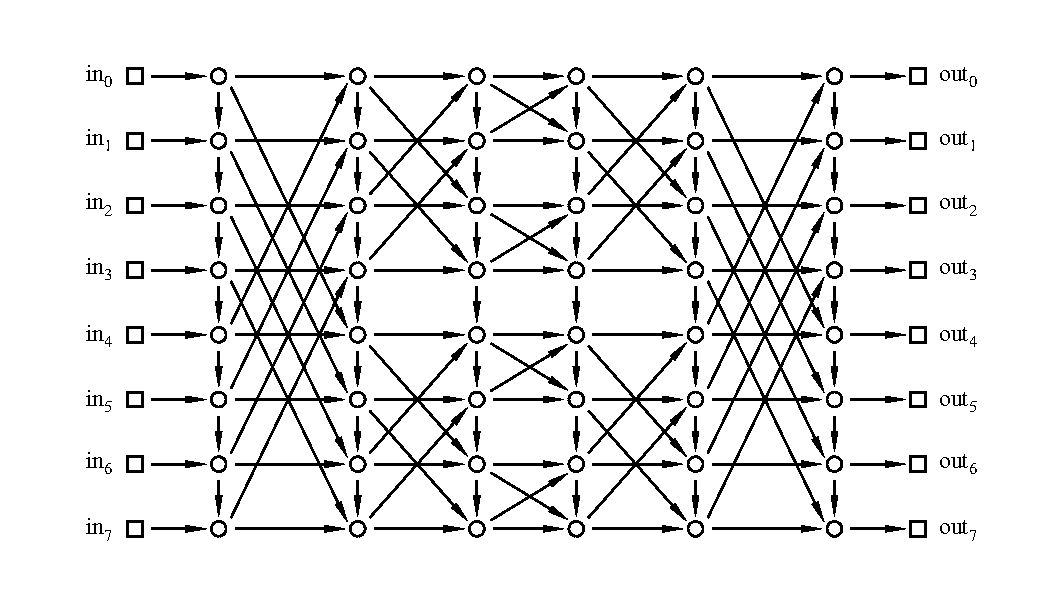
\includegraphics[width=5in]{benes}

\caption{The 8-input Bene\u{s} network.}

\label{fig:6ER}

\end{figure}

Putting two butterflies back-to-back roughly doubles the number of
switches and the diameter of a single butterfly, but it completely
eliminates congestion problems!  The proof of this fact relies on a
clever induction argument that we'll come to in a moment.  Let's first
see how the Bene\u{s} network stacks up against the other networks we
have been studying.  As you can see in Figure~\ref{fig:6ES}, the
Bene\u{s} network has small size and diameter, and completely
eliminates congestion.  The Holy Grail of routing networks is in hand!

\begin{figure}

\begin{tabular}{r|c|c|c|c}
\textbf{network} &
\textbf{diameter} &
\textbf{switch size} &
\textbf{\# switches} &
\textbf{congestion} \\ \hline
complete binary tree & $2 \log N + 2$ & $3 \times 3$ & $2N - 1$ & $N$ \\
2-D array            & $2 N$          & $2 \times 2$ & $N^2$    & 2 \\
butterfly            & $\log N + 2$ & $2 \times 2$ & $N (\log(N) + 1)$
        & $\sqrt{N}$ or $\sqrt{N/2}$ \\
Bene\u{s}           & $2 \log N + 1$ & $2 \times 2$ & $2 N \log N$ & 1
\end{tabular}

\caption{A comparison of the $N$-input Bene\u{s} network with the
  $N$-input complete binary tree, 2-d array, and butterfly.}

\label{fig:6ES}

\end{figure}

\begin{theorem}\label{thm:benes_congestion}
The congestion of the $N$-input Bene\u{s} network is~1 for any $N$
that is a power of~2.
\end{theorem}

\begin{proof}
We use induction.  Let $P(a)$ be the proposition that the congestion of
the $2^a$-input Bene\u{s} network is~1.

\inductioncase{Base case} ($a = 1$): We must show that the congestion
of the $2^1$-input Bene\u{s} network is~1.  The network is shown in
Figure~\ref{fig:6ET}.

\begin{figure}

\missinggraphic

\caption{The 2-input Bene\u{s} network.}

\label{fig:6ET}

\end{figure}

There are only two possible permutation routing problems for a 2-input
network.  If $\pi(0) = 0$ and $\pi(1) = 1$, then we can route both
packets along the straight edges.  On the other hand, if $\pi(0) = 1$
and $\pi(1) = 0$, then we can route both packets along the diagonal
edges.  In both cases, a single packet passes through each switch.

\inductioncase{Inductive step}: We must show that $P(a)$ implies $P(a
+ 1)$ where $a \ge 1$.  Thus, we assume that the congestion of a
$2^a$-input Bene\u{s} network is~1 in order to prove that the
congestion of a $2^{a + 1}$-input Bene\u{s} network is also~1.

\noqed

\end{proof}

\paragraph{Digression}

Time out!  Let's work through an example, develop some intuition, and
then complete the proof.  Notice that inside a Bene\u{s} network of
size~$2N$ lurk two Bene\u{s} subnetworks of size~$N$.  This follows
from our earlier observation that a butterfly of size $2N$ contains
two butterflies of size~$N$.  In the Bene\u{s} network shown in
Figure~\ref{fig:6EU} with $N=8$ inputs and outputs, the two
4-input/output subnetworks are shown in dashed boxes.

\begin{figure}

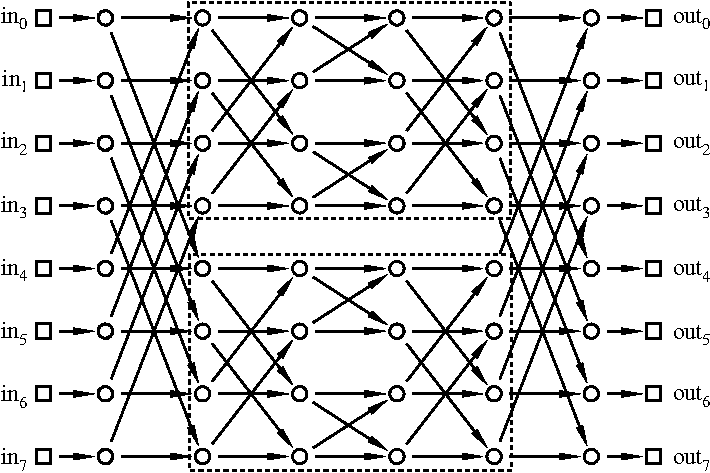
\includegraphics[height=3in]{benes-decomp}

\caption{A $2N$-input Bene\u{s} network contains two $N$-input
  Bene\u{s} networks---shown here for $N = 4$.}

\label{fig:6EU}

\end{figure}

By the inductive assumption, the subnetworks can each route an
arbitrary permutation with congestion 1.  So if we can guide packets
safely through just the first and last levels, then we can rely on
induction for the rest!  Let's see how this works in an example.
Consider the following permutation routing problem:
%
\begin{align*}
\pi(0) & = 1 & \pi(4) & = 3 \\
\pi(1) & = 5 & \pi(5) & = 6 \\
\pi(2) & = 4 & \pi(6) & = 0 \\
\pi(3) & = 7 & \pi(7) & = 2
\end{align*}

We can route each packet to its destination through either the upper
subnetwork or the lower subnetwork.  However, the choice for one
packet may constrain the choice for another.  For example, we can not
route the packets at inputs 0 and~4 both through the same network
since that would cause two packets to collide at a single switch,
resulting in congestion.  So one packet must go through the upper
network and the other through the lower network.  Similarly, the
packets at inputs 1 and 5, 2 and 6, and 3 and 7 must be routed through
different networks.  Let's record these constraints in a graph.  The
vertices are the 8 packets (labeled according to their input
position).  If two packets must pass through different networks, then
there is an edge between them.  The resulting constraint graph is
illustrated in Figure~\ref{fig:6EV}.  Notice that at most one edge is
incident to each vertex.

\begin{figure}

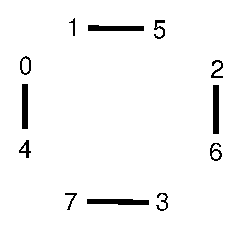
\includegraphics[height=1.5in]{benes-const1}

\caption{The beginnings of a constraint graph for our packet routing
  problem.  Adjacent packets cannot be routed using the same
  sub-Bene\u{s} network.}

\label{fig:6EV}

\end{figure}

The output side of the network imposes some further constraints.  For
example, the packet destined for output 0 (which is packet 6) and the
packet destined for output 4 (which is packet 2) can not both pass
through the same network since that would require both packets to
arrive from the same switch.  Similarly, the packets destined for
outputs 1 and 5, 2 and 6, and 3 and 7 must also pass through different
switches.  We can record these additional constraints in our
constraint graph with gray edges, as is illustrated in
Figure~\ref{fig:6EW}.

\begin{figure}

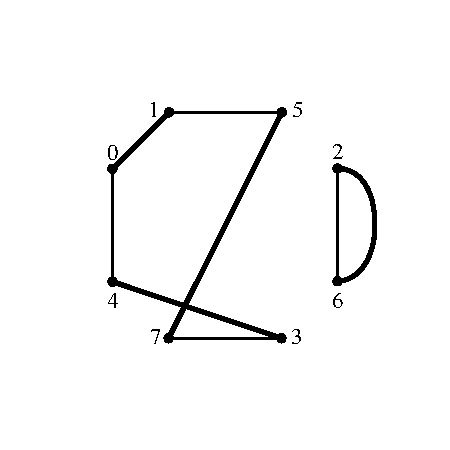
\includegraphics[height=1.5in]{benes-const2}

\caption{The updated constraint graph.}

\label{fig:6EW}

\end{figure}

Notice that at most one new edge is incident to each vertex.
The two lines drawn between vertices 2 and 6 reflect the two different
reasons why these packets must be routed through different networks.
However, we intend this to be a simple graph; the two lines still
signify a single edge.

Now here's the key insight: \emph{a 2-coloring of the graph
corresponds to a solution to the routing problem}.  In particular,
suppose that we could color each vertex either red or blue so that
adjacent vertices are colored differently.  Then all constraints are
satisfied if we send the red packets through the upper network and the
blue packets through the lower network.

The only remaining question is whether the constraint graph is
2-colorable.  Fortunately, this is easy to verify:

\begin{lemma}\label{deg1-union}
  If the edges of an undirected graph~$G$ can be grouped into two sets
  such that every vertex is incident to at most 1 edge from each set,
  then the graph is 2-colorable.
\end{lemma}

\begin{proof}
Since the two sets of edges may overlap, let's call an edge that is in
both sets a \emph{doubled edge}.  Note that no other edge can be
incident to either of the endpoints of a doubled edge, since that
endpoint would then be incident to two edges from the same set.  This
means that doubled edges form connected components with 2 nodes.  Such
connected components are easily colored with 2 colors and so we can
henceforth ignore them and focus on the remaining nodes and edges,
which form a simple graph.

By Theorem~\ref{thm:XY}, we know that if a simple graph has no odd
cycles, then it is 2-colorable.  So all we need to do is show that
every cycle in~$G$ has even length.  This is easy since any cycle
in~$G$ must traverse successive edges that alternate from one set to
the other.  In particular, a closed walk must traverse a path of
alternating edges that begins and ends with edges from different sets.
This means that the cycle has to be of even length.
\end{proof}

For example, a 2-coloring of the constraint graph in
Figure~\ref{fig:6EW} is shown in Figure~\ref{fig:6EX}.  The solution
to this graph-coloring problem provides a start on the packet routing
problem.  We can complete the routing in the two smaller Bene\u{s}
networks by induction.  With this insight in hand, the digression is
over and we can now complete the proof of
Theorem~\ref{thm:benes_congestion}.

\begin{figure}

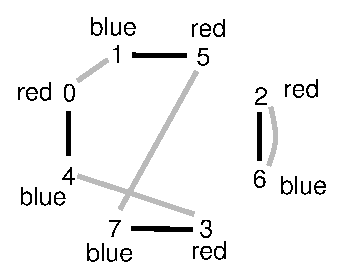
\includegraphics[height=1.75in]{benes-const3}

\caption{A 2-coloring of the constraint graph in
  Figure~\ref{fig:6EW}.}

\label{fig:6EX}

\end{figure}

\begin{proof}[Proof of Theorem \ref{thm:benes_congestion}
    \textup(continued\textup)] 

Let $\pi$ be an arbitrary permutation of 0, 1, \dots, $N-1$.  Let $G$
be the graph whose vertices are packet numbers $0, 1, \dots, N-1$ and
whose edges come from the union of these two sets:
\begin{align*}
E_1 \eqdef &  \set{\, \edge{u}{v} \suchthat \abs{u - v} = N/2 \,},\ \text{and} \\
E_2 \eqdef &  \set{\, \edge{u}{w} \suchthat \abs{\pi(u) - \pi(w)} = N/2\,}.
\end{align*}
Now any vertex, $u$, is incident to at most two edges: a unique edge
$\edge{u}{v} \in E_1$ and a unique edge $\edge{u}{w} \in E_2$.  So
according to Lemma~\ref{deg1-union}, there is a 2-coloring for the
vertices of $G$.  Now route packets of one color through the upper
subnetwork and packets of the other color through the lower
subnetwork.  Since for each edge in $E_1$, one vertex goes to the
upper subnetwork and the other to the lower subnetwork, there will not
be any conflicts in the first level.  Since for each edge in $E_2$,
one vertex comes from the upper subnetwork and the other from the
lower subnetwork, there will not be any conflicts in the last level.
We can complete the routing within each subnetwork by the induction
hypothesis $P(n)$.
\end{proof}

\section{Problems}

\begin{problems}
\examproblems
\pinput{MQ_basic_network_problem}

\classproblems
\pinput{CP_Benes_network}
\pinput{CP_binary-tree_network}
\pinput{CP_2_layer_array_network}
\pinput{CP_n-path_network}
\pinput{CP_Megumi_net}

\homeworkproblems
\pinput{PS_Reasoner_net}
\pinput{PS_butterfly_congestion}
\end{problems}

\iffalse
In class, you will work through an example in which you route packets
using this recursive idea!
\fi

\endinput




\endinput

